\chapter{
  Application
 }
\minitoc%

\section{Généralités}

\subsection{Estimation adaptative informelle}
Les motivations de l'obtention de la régularité étaient en partie de pouvoir mieux estimer les quantités qui nous intéressent dont la fonction moyenne du processus, ainsi que son opérateur de covariance. Ce qui est à la fois important pour l'analyse (via l'interprétation de la base ACP déterminée par la covariance) et pour la prédiction. On peut alors se demander si il existe des estimateurs de la moyenne et de la covariance prenant en compte la régularité locale. C'est ce qu'affirme les théorèmes suivants :

\warn{demander à Hassan la dernière version de son papier car la partie d estimation adaptative a beaucoup changé}

\begin{thm*}[Estimateurs de la moyenne et de la covariance — informel ~\cite{golovkine2021adaptive}]
	\noindent\fbox{%
		\parbox{\textwidth}{%
			Il est possible en lissant les observations par méthode à noyaux avec une largeur de bande \emph{spécifique à l'objet que l'on souhaite estimer}, de dériver des estimateurs de la moyenne et de la covariance qui convergent.
			La largeur de bande optimale \emph{pour l'objet que l'on souhaite estimer} est celle qui minimise un risque qui effectue un compromis biais-variance, qui dépend de la régularité locale du processus, en pénalisant les largeurs de bande menant à des "trous" dans les fonctions lissées.
			On parle d'\emph{\og estimation adaptative \fg}.
		}%
	}

	\label{thm*:estimation_adaptative}
\end{thm*}

Cependant, bien qu'une largeur de bande optimale existe, elle est inconnue. Il est donc important de savoir si le praticien peut l'estimer, et avec quelle précision (c'est à dire à quel point l'estimateur sera biaisé ou non). C'est ce que nous affirme le théorème suivant :

\begin{thm*}[expression de la largeur de bande optimale — informel ~\cite{golovkine2021adaptive}]
	\noindent\fbox{%
		\parbox{\textwidth}{%
			Sous certaines hypothèses de régularité du processus, et d'indépendance des temps observés, la largeur de bande optimale peut être approchée (avec forte probabilité de bonne approximation) par une expression ne dépendant que du nombre de courbes observées, du nombre moyen de temps observés par courbe, et de la régularité locale du processus. Ce biais de l'estimateur de la fonction moyenne est alors contrôlé en fonction de ces mêmes quantités.

			Sous des hypothèses un peu plus fortes sur la relation entre le nombre moyen d'observations par courbe et le nombre de courbes, on dispose de résultats similaires pour l'estimateur de la covariance.}%
	}

	\label{thm*:h_opt_estim}
\end{thm*}


Enfin, on peut se demander ce qu'il en est des estimateurs dans le cadre où l'on dispose de la dépendance dans les données (ce qui est la cas pour les données éoliennes notamment). Ce cas est traîté par le théorème suivant dérivé par MPV :

\begin{thm*}[ Estimation adaptative de séries temporelles fonctionnelles — informel ~\cite{maissoro-SmoothnessFTSweakDep} ]

	On peut estimer la régularité d'une série temporelle de données fonctionnelles à condition que la mémoire temporelle de la série soit courte. (La décroissance de la dépendance temporelle doit être au moins aussi rapide qu'une décroissance géométrique)

	\label{thm*:far_adaptative_estimation}
\end{thm*}

\subsection{Les estimateurs}

\info{ Plus de précisions théoriques sur les estimateurs utilisés sont disponibles dans l'annexe \ref{annexe:estim_adapt}.}

On utilisera les estimateurs considérés par MPV \cite{maissoro-SmoothnessFTSweakDep} pour la fonction moyenne :

\bigskip

\noindent On notera l'indicatrice de l'évènement \og il y a suffisamment de points autour de $t$ pour le lissage à noyaux de la courbe $i$ \fg : $\pi_i(t \, | \, h)$\footnote{On ne demande la présence que d'un unique point, un autre seuil plus strict peut être fixé. Il a été aperçu empiriquement que l'amélioration de l'estimation n'est pas significative, un point suffit pour éviter la dégénérescence.}.

\noindent Le nombre d'observations exploitables dans la bande $J_\Delta$ est donc : $P_N^* =P_N(t \, | \, h_\mu^*(\Delta^*)) = \sum\limits_{i=1}^N \pi_i(t \, | \, h_\mu^*(\Delta^*))$, et de manière équivalente on obtient le nombre d'observations exploitables pour l'estimation conjointe sur les courbes $i$ et $i + \ell$ en $t$: $P_{i,\ell}^*$.

\begin{align}
	\widehat{\mu^*_{\textsf{adapt}}}(t)              & = \frac 1 {P_N^*} \sum_{i=1}^N \left[\pi_i \cdot \widehat X^{[NW]}_i\right]\left(\, t \, | \, h^*_\mu(\Delta^*) \, \right) \\
	\widehat {\gamma^*_{\textsf{adapt}}}(s, t, \ell) & = \frac 1 {P^*_{i, \ell}}\sum_{i=1}^{N- \ell} \left[
		\left[\pi_i \cdot \widehat X^{[NW]}_i\right]\left(\, s \, | \, h^*_\mu(\Delta^*) \, \right) \left[\pi_{i + \ell} \cdot \widehat X^{[NW]}_{i + \ell}\right]\left(\, t \, | \, h^*_\mu(\Delta^*) \, \right)
		\right]                                                                                                                                                                       % \\
	% \widehat {C^*_{\textsf{adapt}}}(s,t)             & = \widehat {\gamma^*_{\textsf{adapt}}}(s, t, \ell) -
	% \widehat{\mu^*_{\textsf{adapt}}}(s)\widehat{\mu^*_{\textsf{adapt}}}(t)
\end{align}

On établit désormais si la procédure de détermination du $\Delta$ établie en section [\ref{sec:determination-delta}] permet bel et bien d'obtenir une bonne estimation des paramètres de régularité sur de nouvelles données générées.

\section{Contrôle de la procédure sur des données simulées}

Il est important que les données de test n'aient pas été utilisées pour déterminer la procédure. Pour vérifier que la procédure fonctionne comme prévu, on génère de nouvelles données aux caractéristiques suivantes :


\begin{table}[H]
	\centering
	\begin{tabularx}{\textwidth}{XXXX}
		\toprule
		\textbf{Nombre moyen d'observations par courbe}     & \textbf{symbole}                & \textbf{variation} & \textbf{valeur}                                           \\
		\bottomrule
		\multirow{3}{\hsize}{Nombre moyen d'observations}   & \multirow{3}{\hsize}{$\lambda$} & sparse             & 80                                                        \\
		                                                    &                                 & moyen              & 180                                                       \\
		                                                    &                                 & dense              & 300                                                       \\
		\midrule
		\multirow{3}{\hsize}{Nombre de courbes}             & \multirow{3}{\hsize}{$N$}       & sparse             & 100                                                       \\
		                                                    &                                 & moyen              & 200                                                       \\
		                                                    &                                 & dense              & 300                                                       \\
		\midrule
		Nombre de simulations de monte carlo                & $mc$                            &                    & 200                                                       \\
		\midrule
		Points d'estimation de la régularité                & $\vec t$                        &                    & $[0.3, 0.6, 0.8]$                                         \\
		\midrule
		\multirow{2}{\hsize}{Fonction de Hurst}             & $H_1$                           & même que sim       & $t \mapsto H^{[0.4, 0.8, 5, 0.5]}_{\textsf{logistic}}(t)$ \\
		                                                    & $H_2$                           & pente plus abrupte & $t \mapsto H^{[0.4, 1, 16, 0.6]}_{\textsf{logistic}}(t)$  \\
		\\
		\multirow{2}{\hsize}{Valeurs de régularité testées} & $H_1\bigl( \, \vec t \, \bigr)$ & même que sim       & $\bigl[ \, 0.51, 0.65, 0.73 \, \bigr]$                    \\
		                                                    & $H_2\bigl( \, \vec t \, \bigr)$ & pente plus abrupte & $\bigl[ \, 0.40, 0.70, 0.98 \, \bigr]$                    \\
		\midrule
		constante de régularité locale                      & $L_t$                           & constante          & 3                                                         \\
		\bottomrule
	\end{tabularx}
	\caption{Paramètres de simulation des données de test}
	\label{tab:sim_test_params}
\end{table}

\noindent Puis on estimera la régularité de chacune de ces courbes, et on comparera les résultats obtenus avec les valeurs théoriques.

\subsection{Détermination du $\Delta$ en utilisant la procédure}

Nous choisissons, en accord avec la section précédente, le $\Delta$ suivant :

\begin{equation*}
	\Delta^{proc} = 15\% \textsf{ du support} \,  .
\end{equation*}

% \subsection{Estimation de la fonction moyenne}

% On compare désormais les fonctions moyennes estimées de façon adaptative avec la fonction moyenne théorique en ayant effectué une estimation de la régularité avec $\Delta = \Delta^{proc}$ et $h = h^{[cv(\widehat \lambda)]}$.

% \editlater{graphe de la fonction moyenne estimée contre la véritable fonction moyenne}

\subsection{Conclusion sur la qualité de la détermination du $\Delta$ via l'utilisation de la procédure}

\noindent De la même manière que dans l'annexe \ref{annexe:choix-du-rique}, on retire sur les 200 échantillons de monte carlo simulés, les échantillons \og extrêmes \fg où une observation peut potentiellement faire exploser le risque (auquel cas on rappelle que l'on conseille la méthode de Golovkine et al. (2022) par la statistique d'ordre si les résultats sont insatisfaisants sur le voisinage problématique). On note $\textsf{mc}_{Ret}$ le nombre de simulations de Monte-Carlo retenues dans le calcul après filtrage des \og extrêmes \fg.

\bigskip

\noindent Les risques affichés par la suite sont pour $N=200$, $\lambda = 180$.\footnote{Les tableaux de risque pour les autres valeurs mentionnées précédemment sont disponibles en annexe} On considère l'estimation du couple

\begin{minipage}{0.45\textwidth}
	\begin{equation*}
		\widetilde \thetaB = \begin{bmatrix} \widetilde \theta(t_1, t_3)\\ \widetilde \theta(t_2, t_3) \end{bmatrix}
	\end{equation*}
\end{minipage}
\begin{minipage}{0.45\textwidth}
	Que l'on estime avec $\widehat \thetaB = \begin{bmatrix} \widehat \theta(t_1, t_3)\\ \widehat \theta(t_2, t_3) \end{bmatrix}$
\end{minipage}

\bigskip

\subsubsection{Qualité d'estimation du couple d'incréments $\tilde \thetaB$ : risque relatif}

\begin{table}[H]
	\centering
	\begin{tabularx}{\linewidth}{|X|X|XX|X|X|}
		\toprule
$t$                                  & $H_t$        & $\widehat{\mathcal R}^{[\,rel\,]}(\Theta, \Delta)$ & $\textsf{mc}_{Ret}$ & $\mathbf{\operatorname{med}\widehat{\mathcal R}^{[\,rel\,]}_{mc}(\Theta, \Delta)}$ & $\mathbf{\mathds V[\widehat{\mathcal R}^{[\,rel\,]}_{mc}(\Theta, \Delta)]}$ \\
		\midrule
		\multirow{2}{\hsize}{Moins Régulier} & $H_1 : 0.51$ & 2.9 $\cdot 10^{-3}$                    & $\vdots$            & 2.3 $\cdot 10^{-3}$                                                    & 5.0 $\cdot 10^{-6}$
		\\
		                                     & $H_2 : 0.40$ & 7.8 $\cdot 10^{-3}$                    & $\vdots$            & 5.1 $\cdot 10^{-3}$                                                    & 1.1 $\cdot 10^{-4}$
		\\
		\midrule
		\multirow{2}{\hsize}{Inflexion}      & $H_1 : 0.65$ & 9.0 $\cdot 10^{-5}$                    & $\vdots$            & 4.9 $\cdot 10^{-5}$                                                    & 1.2 $\cdot 10^{-8}$
		\\
		                                     & $H_2 : 0.70$ & 1.5 $\cdot 10^{-3}$                    & 198 (/200)          & 5.0 $\cdot 10^{-5}$                                                    & 2.3 $\cdot 10^{-4}$
		\\
		\midrule
		\multirow{2}{\hsize}{Plus régulier}  & $H_1 : 0.73$ & 1.1 $\cdot 10^{-4}$                    & $\vdots$            & 6.7 $\cdot 10^{-5}$                                                    & 1.5 $\cdot 10^{-8}$
		\\
		                                     & $H_2 : 0.98$ & 2.3 $\cdot 10^{-3}$                    & $\vdots$            & 7.8 $\cdot 10^{-5}$                                                    & 3.1 $\cdot 10^{-4}$
		\\
		\bottomrule
	\end{tabularx}
	\label{tab:qualite_estim_increments_relatif_new_sim}
	\caption{Table du risque relatif sur l'estimation du couple $\widetilde\thetaB$ pour $\lambda=180, N=200$}
\end{table}

\noindent\chk{On peut constater que les risques relatifs observés sur l'estimation du couple $\tilde \thetaB$ pour de tous nouveaux paramètres de simulation sur lesquels la procédure de sélection du $\Delta$ n'a pas été déterminée ($H_2$) sont aussi très bons ce qui donne confiance en la procédure.}

\subsection{Qualité d'estimation de la régularité}

\begin{figure}[H]
	\centering
	$N = 200$, $\lambda = 180$ | $\widehat{\mathcal R}(t) = \frac 1 {mc} \sum\limits_{i=1}^{mc} (\widehat{H_t}[i] - H_t)^2$

	\centering
	\noindent\begin{minipage}{0.32\linewidth}
		\centering
		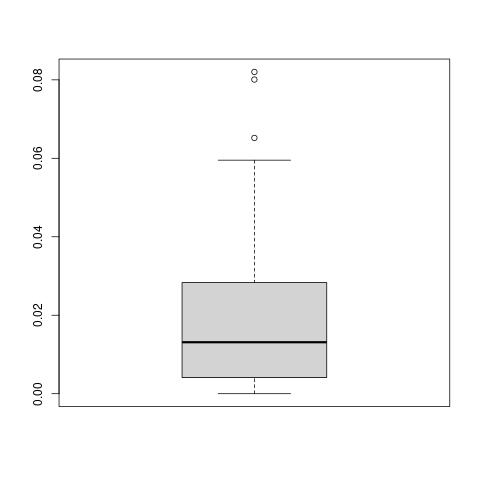
\includegraphics[width=\textwidth]{Images/N200_lbd180_box3_2.jpg}
		moins régulier : H = 0.40
	\end{minipage}
	\begin{minipage}{0.32\linewidth}
		\centering
		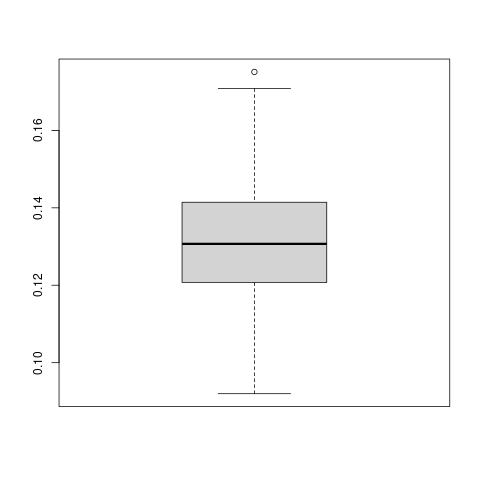
\includegraphics[width=\textwidth]{Images/N200_lbd180_box6_2.jpg}
		inflexion : H = 0.70
	\end{minipage}
	\begin{minipage}{0.32\linewidth}
		\centering
		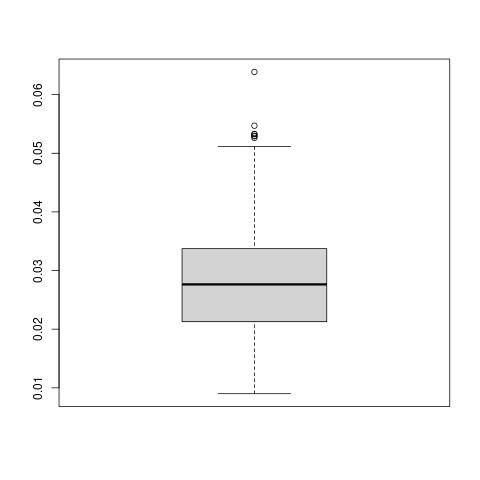
\includegraphics[width=\textwidth]{Images/N200_lbd180_box8_2.jpg}
		plus régulier : H = 0.98
	\end{minipage}
	\caption{Distribution des risques sur l'estimation du paramètre de régularité locale : $H_t$}
	\label{fig:H_error_boxplot}
\end{figure}

\pagebreak

\subsection{Qualité d'estimation de la fonction moyenne : Critère Local}

Nous nous intéressons désormais à la qualité d'estimation de la fonction moyenne en respectant la procédure décrite précédemment pour la sélection du $\Delta$.

\begin{table}[H]
	\centering
	\begin{tabularx}{\linewidth}{|X|X|X|X|X|X|X|}
		\toprule
		$t$                                  & $H_t$        & $\widehat{\mathcal R}(t)$ avec $\mathcal R$ = MSE & $\mathbf{\operatorname{med}(\widehat{\mathcal R}_{mc}(t))}$ & $\mathbf{\mathds V[\widehat{\mathcal R}_{mc}(t)]}$ & $N$                       & $\lambda$
		\\
		\midrule
		\multirow{2}{\hsize}{Moins régulier} & $H_1 : 0.51$ & 5.4 $\cdot 10^{-3}$                               & 2.6  $\cdot 10^{-3}$                                        & 5.5$\cdot 10^{-5}$                                 & \multirow{6}{\hsize}{200} & \multirow{6}{\hsize}{180}
		\\
		                                     & $H_2 : 0.40$ & 1.4$\cdot 10^{-2}$                                & 5.0$\cdot 10^{-3}$                                          & 4.4$\cdot 10^{-4}$                                 &                           &
		\\
		\cmidrule{1-5}
		\multirow{2}{\hsize}{Inflexion}      & $H_1 : 0.65$ & 8.0$\cdot 10^{-3}$                                & 4.4$\cdot 10^{-3}$                                          & 8.2$\cdot 10^{-5}$                                 &                           &
		\\
		                                     & $H_2 : 0.70$ & 3.5$\cdot 10^{-2}$                                & 1.8$\cdot 10^{-2}$                                          & 2.7$\cdot 10^{-3}$                                 &                           &
		\\
		\cmidrule{1-5}
		\multirow{2}{\hsize}{Plus régulier}  & $H_1 : 0.73$ & 5.2$\cdot 10^{-3}$                                & 2.5$\cdot 10^{-3}$                                          & 4.3$\cdot 10^{-5}$                                 &                           &
		\\
		                                     & $H_2 : 0.98$ & 4.0$\cdot 10^{-2}$                                & 1.8$\cdot 10^{-2}$                                          & 2.8$\cdot 10^{-3}$                                 &                           &
		\\
		\bottomrule
	\end{tabularx}
	\caption{Risques quadratiques (MSE) de l'estimation adaptative de la fonction moyenne}
\end{table}

\subsection{Conclusion sur la validité de la procédure de sélection du $\Delta$}

\chk{
	\smallskip\centering
	L'analyse des risques sur l'estimation du paramètre de régularité $H_t$ ainsi que sur l'estimation de la fonction moyenne $\mu$ sur des données simulées avec de nouveaux paramètres semble indiquer que la procédure de sélection du $\Delta$ fonctionne comme prévu.
}

\noindent 
\begin{center}
\fbox{%
\begin{adjustbox}{minipage=\linewidth}
	\noindent \blueboxed{\faPen \, commentaire (personnel) } Il aurait été judicieux de considérer une fonction de Hurst décroissante (en inversant $h_\ell$ et $h_r$ dans la définition de $H_t$), pour vérifier l'indépendance de la méthode vis-à-vis du sens de monotonicité de celle-ci. Une autre expérience possible serait considérer une fonction non monotone et de regarder en un point de croissance et en un point de décroissance (de pente opposée).
\end{adjustbox}
}
\end{center}

\section{
  Application sur les données réelles de courbes de charge éolienne et photovoltaïque
 }

\subsection{Présentation des jeux de données}

Les données que l'on traîte sont des courbes de charge provenant de différents moyens de production : éolien ou photovoltaïque. Comme mentionné en section \ref{sec:func_ts}, il y a plusieurs façons de découper les données observées pour les modéliser par des données fonctionnelles : identifiant, temporel, ... Nous allons ici illustrer cet aspect en présentant deux jeux de données : un jeu de données éoliennes et un jeu de données photovoltaïques. Nous modélisons les données éoliennes de la façon suivante :

\bigskip

\noindent\begin{tabularx}{\textwidth}{XX}
	\toprule
	\textbf{Données éoliennes}                                                                                                                                                                              \\
	\midrule
	support            & année identifiée comme $\mathcal T = [0,1]$                                                                                                                                        \\
	modèle fonctionnel & $\forall i \in I \quad E_i : \func {\Omega \times [0,1]} {\mathds R_+} {(\omega, t)} {e_i(t)}$                                                                                     \\
	indices            & éolienne individuelle : $I = \bigl\{ \, \textsf{id du parc éolien} \,\bigr\}$                                                                                                      \\
	\\
	observations       & $\widehat E = \bigl\{ \, (T_i[m], Y_i[m]) \, : \, i \in \intervaleint 1 N, m \in \intervaleint 1 {M_i} \bigr\}$ : $Y_i[m] = E_i\bigl( \, T_i[m] \, \bigr) + \eta_i\bigl[ m \bigr]$ \\
	\\
	erreur de mesure   & $(\eta_i[m])_{I\times\llbracket 1, M_i \rrbracket}$ : indépendants 2 à 2                                                                                                           \\
	\\
	dépendance         & données indépendantes car les éoliennes ne s'influencent pas sur leur production.                                                                                                  \\
	\bottomrule
\end{tabularx}

\bigskip

% Toutefois, les résultats que nous allons désormais présenter concernent le jeu de données de production électrique de panneaux photovoltaïques. Ici, contrairement aux données éoliennes, on dispose d'une courbe de charge d'un unique parc photovoltaïque. La courbe de charge a été observée toutes les demie-heures pendant un an. Nous sommes donc sur un schéma de \og common-design \fg. Étant donné la présence d'un \og cycle de production \fg qui semble se répéter chaque jour, on décide de les modéliser par des séries temporelles fonctionnelles. Chaque courbe représente une journée, on dipose donc de 365 courbes dont le support représente une journée. Pour résumer :
Nous allons maintenant présenter les résultats obtenus sur le jeu de données de production électrique photovoltaïque. Cette fois-ci, nous traîtons qu'un unique parc photovoltaïque et \emph{une journée} de production est représentée par \emph{une courbe}. L'ensemble des courbes sont observées toutes les 30 minutes (suivant donc un schéma de \og common design \fg). On dispose au total d'une année de données, soit 365 courbes. En résumé :

\bigskip

\noindent\begin{tabularx}{\textwidth}{XX}
	\toprule
	\textbf{Données Photovoltaïques}                                                                                                                                                                       \\
	\midrule
	support            & heure du jour identifiée comme $\mathcal T = [0,1]$                                                                                                                               \\
	\\
	modèle fonctionnel & ${V}_i : \func {\Omega \times [0,1]} {\mathds R_+} {(\omega, t)} {v_i(t)}$                                                                                                        \\
	\\
	indices            & jour de l'année : $I = \, \llbracket 1, 365 \rrbracket$                                                                                                                           \\
	\\
	observations       & $\widehat V = \bigl\{ \, (T_i[m], Z_i[m]) \, : \, i \in \intervaleint 1 N, m \in \intervaleint 1 {M_i} \bigr\}$ : $Z_i[m] = V_i\bigl( \, T_i[m] \, \bigr) + \eta_i\bigl[ m \bigr]$ \\
	\\
	erreur de mesure   & $\eta_i$ : indépendants 2 à 2                                                                                                                                                     \\
	\\
	dépendance         & série temporelle fonctionnelle : même parc, courbes journalières cycliques, indice temporel, observation dans le temps                                                                               \\
	\\
	\bottomrule
\end{tabularx}

\bigskip

\begin{rem}
	On pourra constater que les données éoliennes et les données photovoltaïques rendent compte de la remarque faite en section \ref{sec:func_ts} : l'un des jeux de données est indexé sur le temps, l'autre sur un identifiant. De plus les données photovoltaïques présentent à la fois un indice et un support temporel.
\end{rem}


\subsection{Pré-traitement des données}

La manipulation des séries temporelle requiert la stationnarité. Hors, la moyenne de production électrique des panneaux solaires varie dans l'année (durée des journées, fréquence de pluies, ...). Ainsi on découpe le jeu de données selon la saison, dans la suite du rapport nous nous concentrerons sur la courbe de charge pendant la période estivale (on pose donc $\bigl[ \, 21/06/2017, \, 22/09/2017 \, ] = \mathcal T \isdef \bigl[ 0, 1 \bigr]$). Enfin, on décide de ne pas estimer sur l'ensemble de la journée, mais pendant la période de production électrique effective, et donc nous retirons de l'estimations les horaires de nuit qui se situe selon les données observées de 21h à 6h. En effet, la production électrique pendant ces horaires est nulle et n'a pas besoin d'être estimée (on pourra se référer à la figure \ref{fig:boxplot_pv_journee}).


\subsection{Estimation de la régularité locale et de la fonction moyenne}


L'estimation des paramètres de régularité $H$ et $L$  qui varient sur le support nous permet d'une part de prendre en compte la régularité du processus pour l'estimation de la fonction moyenne, mais aussi d'autre part de pouvoir comparer la régularité de la production électrique lors de différentes saisons.
On remarque bien que la production d'électricité en moyenne est nettement inférieure en hiver qu'en été, en plus de voir le pic de production légèrement plus tôt en Hiver, peu après midi.
On constate de plus que la production électrique est bien plus irrégulière en hiver qu'en été comme on pouvait s'y attendre : Les valeurs de $H$ sont plus souvent en dessous de $0.5$ en hiver qu'en été et vartie fortement sur l'ensemble du support sans se stabiliser. 

\begin{figure}[H]
	\centering
	% PRINTEMPS
	\begin{minipage}{0.48\textwidth}
	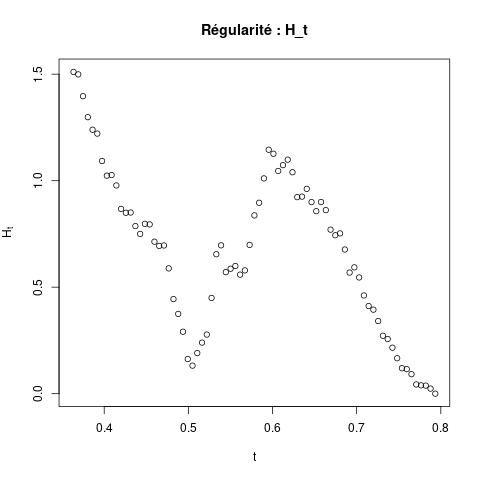
\includegraphics[width=0.89\textwidth]{Images/pv_estim/hiv_187128_Ht.jpg}
	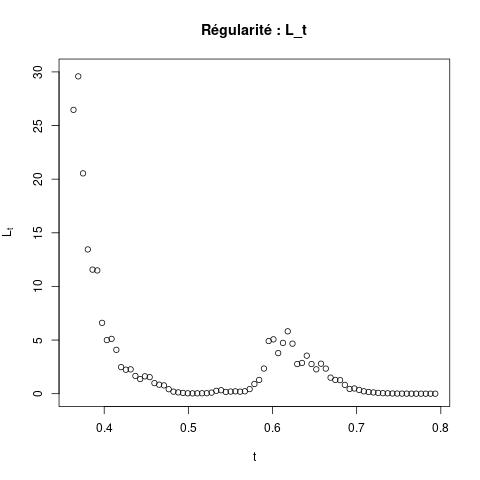
\includegraphics[width=0.89\textwidth]{Images/pv_estim/hiv_187128_Lt.jpg}
	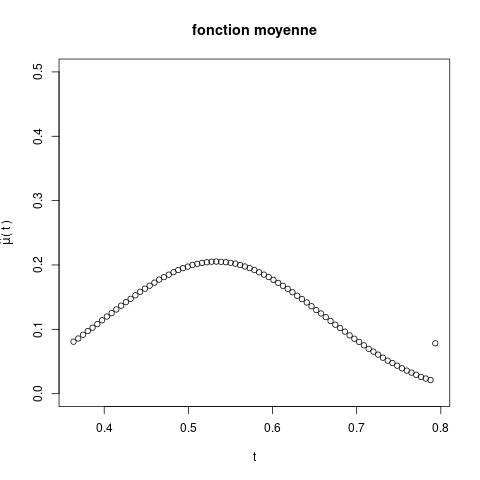
\includegraphics[width=0.89\textwidth]{Images/pv_estim/hiv_187128_mut.jpg}
	\end{minipage}
	% TODO : mêmes images, mettre à la place les images d une autre saison
	% \hfill
	\begin{minipage}{0.48\textwidth}
		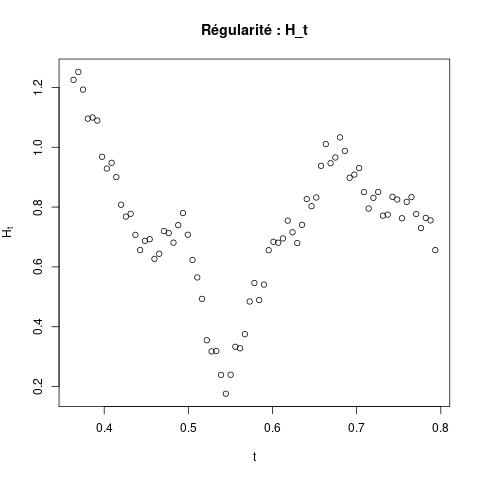
\includegraphics[width=0.89\textwidth]{Images/pv_estim/ete_187128_Ht.jpg}
		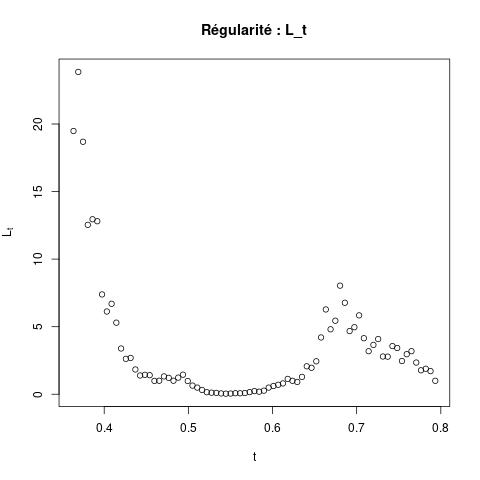
\includegraphics[width=0.89\textwidth]{Images/pv_estim/ete_187128_Lt.jpg}
		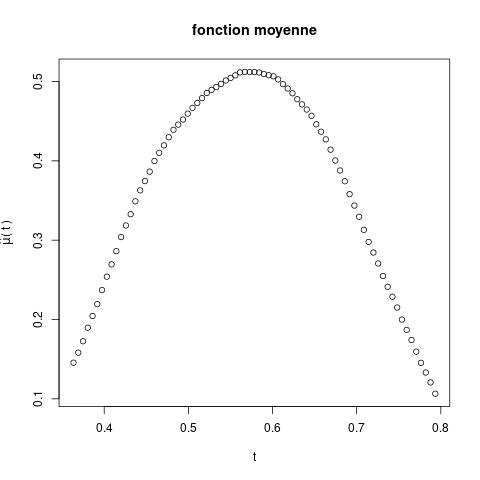
\includegraphics[width=0.89\textwidth]{Images/pv_estim/ete_187128_mut.jpg}
	\end{minipage}
	\begin{minipage}{0.48\textwidth}
		\centering
		Hiver
	\end{minipage}
	\begin{minipage}{0.48\textwidth}
		\centering
		Été
	\end{minipage}
	\caption{Comparaison de l'estimation de la régularité et de la fonction moyenne sur les données photovoltaïques sur un même parc entre l'hiver et l'été}
	\label{fig:estim_reg_mu_hiv_ete}
\end{figure}


\chapter{Conclusion}

Les données fonctionnelles constituent un paradigme intéressant pour l'analyse des courbes de charge. Si la théorie semble parfois être plus compliquée que celle dont on a l'habitude sur des données à valeurs dans $\mathds R^d$, elle suit néanmoins les mêmes grandes idées et principes que l'on a l'habitude de voir. Les données fonctionnelles devraient donc être accessibles aux statisticiens. Cette modélisation permet notamment de pouvoir extraire la régularité des trajectoires observées du processus que l'on étudie. 

\bigskip

Une telle modélisation permet de prendre en compte de nombreuses caractéristiques des données. Parmi ces caractéristiques il y a notamment la régularité. La prise en compte de la régularité répond à plusieurs problématiques auxquelles le statisticien est souvent confronté : 

\begin{itemize}
	\item \textbf{Performance des prédictions :} savoir bien prédire des valeurs inobservées (potentiellement futures) est un enjeu majeur et critique de nombreuses applications. N'importe quel gain de performance peut s'avérer être un avantage concurrentiel non négligeable. Dans le cadre de la prise en compte de la régularité des trajectoires pour l'estimation de quantités pour des données fonctionnelles, l'amélioration de l'estimation peut s'avérer drastique en fonction de l'objet considéré. ($\emphcolor{cf}$ \cite{golovkine2021adaptive} et \cite{wei2023adaptive} pour l'estimation de la covariance).
	\item \textbf{Interprétabilité \& confrontation du modèle à la réalité :} modéliser un processus fondamentalement (du moins lorsque l'on a de bonnes raisons de le penser) non dérivable par des courbes $\mathcal C^\infty$ ne semble pas être judicieux et impacte l'interprétabilité et la confiance en le modèle.
	\item \textbf{Analyse :} l'estimation de la régularité nous donne directement un nouvel outil pour essayer de comprendre les phénomènes que nous étudions en statistique. Ce n'est pas seulement un intermédiaire pour obtenir une bonne prédiction, mais aussi une source de nouvelles informations qui peuvent servir à analyser un phénomène et prendre des décisions. Si dans le cadre des courbes de charge photovoltaïques on pouvait se douter de la forme des paramètres de régularité, qu'en est-t-il des phénomènes dont on ne fait pas l'expérience sensorielle aussi fréquemment que la météo ? Dans certains phénomènes physiques, ou chimiques ayant des applications industrielles, l'analyse des courbes des paramètres de régularité sur le support peut permettre de mettre en évidence des phénomènes physiques ou chimiques qui n'auraient pas été mis en évidence par une analyse des courbes brutes.
\end{itemize}

\bigskip

Bien que la théorie des données fonctionnelles avec la prise en compte de la régularité des trajectoires soit encore aujourd'hui en pleine construction, il est d'ores et déjà possible de pouvoir estimer de nombreuses quantités prenant en compte cette régularité. Entre autres, nous pouvons mentionner les paramètres de régularité locale, la fonction moyenne, la covariance et même le noyau de la relation d'autorégression d'un modèle de séries temporelles fonctionnelles. Ces méthodes sont même implémentées dans le package R \mintinline{R}{AdaptiveFTS} dérivé des travaux de MPV~\cite{maissoro-SmoothnessFTSweakDep}; et l'étude lors de ce stage de l'hyper-paramètre $\Delta$ utilisé pour l'estimation de la régularité locale permettra désormais au praticien de pouvoir exploiter pleinement ces méthodes.
